% mainfile: ../../main.tex
\chapter{Theory of spectral noise estimation}\label{ch:speck:theory}
\AutoLettrine{There} exist various methods for estimating the properties of noise in a classical signal $x(t)$.\sidenote{
    We discuss only classical noise here, meaning $x(t)$ commutes with itself at all times. For descriptions of and spectroscopy protocols for quantum noise refer to \citerr{Clerk2010}{Paz-Silva2017}, for example.
}
A simple metric quantifying the average noise amplitude of the signal observed from time $t=0$ to $t=T$ is the \gls{rms}~\cite{RMSMathworld},
\begin{align}\label{eq:speck:rms:timedomain}
    \rms_x = \sqrt{\frac{1}{T}\int_{0}^{T}\dd{t}\abs{x(t)}^2}.
\end{align}
While this already tells us \emph{something} about the noise, it is evident that a single number does not provide many clues if we were to attempt to mitigate the noise or say something qualitative about it beyond \enquote{small} and \enquote{large}.
In cases such as these, physics has often turned to the \emph{spectral} representation of the function of interest.
Knowing the frequency content of a function gives access to a wealth of information about the underlying contributing processes.
But how can we learn how a system behaves as a function of frequency?

\begin{marginfigure}[*-6]
    \centering
    \begin{circuitikz}[every node/.style={font=\sffamily\small}]
    % Draw the lock-in amplifier block
%    \node[draw, minimum width=1cm, minimum height=0.5cm, align=center] (lockin) at (0,1) {\acrshort{lia}};
    \node[draw, minimum width=1cm, minimum height=0.5cm, align=center] (lockin) at (-1,0) {\acrshort{lia}};

    % Draw the DUT (device under test)
%    \node[draw, minimum width=1cm, minimum height=0.5cm, align=center] (dut) at (0,-1) {\acrshort{dut}};
    \node[draw, minimum width=1cm, minimum height=0.5cm, align=center] (dut) at (1,0) {\acrshort{dut}};

    % Connection: Lock-In output --> DUT input
%    \draw[->, thick] (lockin.south west) to[bend right=45] node[midway, sloped, below] {$V(t)$} (dut.north west);
    \draw[->, thick] (lockin.north) to[bend left=60] node[midway, sloped, above] {$V(t)$} (dut.north);

    % Connection: DUT output --> Lock-In input
%    \draw[->, thick] (dut.north east) to[bend right=45] node[midway, sloped, below] {$I(t)$} (dut.north east |- lockin.south east);
    \draw[->, thick] (dut.south) to[bend left=60] node[midway, sloped, below] {$I(t)$} (lockin.south);
\end{circuitikz}
    \caption[\imgsource{img/tikz/spectrometer/lockin_dut.tex}]{Measuring the conductance through a \gls{dut} using a \gls{lia}.}
    \label{fig:speck:theory:lockin_dut}
\end{marginfigure}

Consider an electrical black box -- some \acrfull{dut} -- with two leads connected to a \acrfull{lia} as sketched in \cref{fig:speck:theory:lockin_dut}.
Assuming the \gls{dut} is conducting, we could simply measure the conductance $G(t) = \flatfrac{I(t)}{V(t)}$ through the device for some time $T$ with a given lock-in modulation frequency $f_i$, subtract the constant offset,\sidenote{
    The constant part $G_0 = G(t) - \delta G(t)$ of course also holds some information about the system, for example about its bandwidth.
}
and calculate the \gls{rms} using \cref{eq:speck:rms:timedomain}.
Repeating this procedure for different modulation frequencies \set{f}{i}, we would collect a set of \gls{rms}-values that we could assign to the modulation frequencies at which they were measured and thus sample the noise amplitude spectrum\sidenote{
    We will properly define this term below.
}
of the conductance, $S_G(f_i)$.\sidenote{
    See \cref{subsec:speck:software:features:serial} for a discussion on how the \gls{rms} at a certain frequency relates to other quantities discussed in this part.
}
This method has the advantage that we can choose the frequencies at which the spectrum should be sampled---in particular they do not have to be evenly spaced.
However, it has two significant shortcomings.
First, it is rather inefficient and therefore time-consuming.
For $N$ frequency sample points, it takes a total time of $NT$ to acquire all data, where $T$ needs to be chosen such that the variance of $\rms_G$ is sufficiently small.
Second, and crucially, it is not always possible to excite the system at a certain frequency and measure its response.
For example, it is generally considered hard\sidenote{
    And also unpopular with colleagues.
}
to -- deliberately -- excite vibrations of a specific frequency in a cryostat, yet we might still be interested in the displacement spectrum inside of it.
A related method is available if one has access to a frequency-tunable probe, that is, a physical system whose behavior -- typically its time evolution or some measurable property after letting the system evolve -- under noise is well understood within a given noise model, and that can be controlled to be sensitive to a certain frequency.
One example for such methods is \gls{dd}-based noise spectroscopy using a qubit~\cite{Alvarez2011,Szankowski2017,Dial2013,Connors2022}, a protocol based on insights gained from the filter-function formalism---see \cref{part:ff}.
These protocols are especially well-suited for high but less so for low frequencies as they rely on observing the coherence of a qubit and hence the visibility on long time scales.

In a sense the most straight-forward way of measuring the noise spectrum presents itself as a consequence of the Wiener-Khinchin theorem~\cite{Wiener1930,Khintchine1934} that relates the noise spectrum to the Fourier transform of a time-dependent signal.
This makes it possible to estimate the noise spectrum by simply observing a signal for a certain amount of time and performing some post-processing!\sidenote{
    An interesting combination of the Fourier-transform-based and the qubit-based spectroscopy methods was recently proposed in \citer{Vezvaee2024}, where they compute the spectrum by Fourier-transforming the second derivative of the coherence function.
}
This method will be the topic of the present chapter.
It is laid out as follows.
I will first derive the Wiener-Khinchin theorem for continuous stochastic processes and introduce the central quantity of interest in noise spectroscopy; the \gls{psd}.
Then, I will discretize the method and discuss resulting side-effects before describing an efficient way of obtaining the spectrum from a finite amount of data.
Finally, I elaborate on relevant parameters and properties.

\section{Spectrum estimation from time series}\label{sec:speck:theory:time_series_estimation}
To see how spectral noise properties may be estimated from time series data, consider a continuous wide-sense stationary\sidenote{
    \label{sidenote:speck:autocorrelation}
    For a wide-sense stationary (also called weakly stationary) process $x(t)$, the mean is constant and the autocorrelation function $C(t, t') = \ev{x(t)\conjugate x(t^\prime)}$ simplifies to $\ev{x(t)\conjugate x(t + \tau)} = \ev{x(0)\conjugate x(\tau)}$ with $\tau = t^\prime - t$.
    That is, it is a function of only the time lag $\tau$ and not the absolute point in time.
    For Gaussian processes as discussed here, this also implies stationarity~\cite{Koopmans1995}.
    The property further implies that $C(\tau)$ is an even function.
}
signal in the time domain, $x(t)\in\mathbb{C}$, that is observed for some time $T$.
We define the windowed Fourier transform of $x(t)$ and its inverse by\sidenote{
    In this chapter we will always denote the Fourier transform of some quantity $\xi$ using the same symbol with a hat, $\hat{\xi}$.
}
\begin{align}
    \hat{x}_T(\omega) &= \int_{0}^{T}\dd{t} x(t)\e^{-\i\omega t} \label{eq:speck:windowed_ft}\\
       \qq*{and} x(t) &= \intinf\ddf{\omega}\hat{x}_T(\omega)\e^{\i\omega t}, \label{eq:speck:windowed_ft:inverse}
\end{align}
\ie, we assume that outside of the window of observation $x(t)$ is zero.
The autocorrelation function of $x(t)$ is given by
\begin{align}
    C(\tau) &= \expval{x(t)\conjugate x(t + \tau)} \label{eq:speck:autocorrelation}\\
            &= \lim_{T\to\infty} \frac{1}{T}\int_0^T\dd{t} x(t)\conjugate x(t + \tau),
\end{align}
where $\expval{\placeholder}$ is the ensemble average over multiple realizations of the process and the last equality holds true for ergodic processes.
Expressing $x(t)$ in terms of its Fourier representation (\cref{eq:speck:windowed_ft}) and reordering the integrals, we get\sidenote{
    Mathematicians might at this point argue the integrability of $x(t)$, but as we deal with physical processes with finite bandwidth -- and have no shame --, we do not.
}
\begin{align}
    C(\tau) &= \lim_{T\to\infty}\frac{1}{T}\int_0^T\dd{t}
                \intinf\ddf{\omega}\hat{x}_T(\omega)\conjugate\e^{-\i\omega t}
                \intinf\ddf{\omega^\prime}\hat{x}_T(\omega^\prime)\e^{\i\omega^\prime (t + \tau)}  \\
            &= \lim_{T\to\infty}\frac{1}{T}\intinf\ddf{\omega}\intinf\ddf{\omega^\prime}
                \hat{x}_T(\omega)\conjugate\hat{x}_T(\omega^\prime)\e^{\i\omega^\prime\tau}
                \int_0^T\dd{t}\e^{\i t (\omega^\prime - \omega)} \label{eq:speck:autocorrelation:fourier}
\end{align}
The innermost integral approaches a $\delta$-function for large $T$,\sidenote{
    Note that, because $x(t)$ is wide-sense stationary, we may shift the limits of integration $\int_{0}^{T}\to\int_{-\flatfrac{T}{2}}^{+\flatfrac{T}{2}}$.
}
allowing us to further simplify this under the limit as
\begin{align}
    C(\tau) &= \lim_{T\to\infty} \frac{1}{T}\intinf\ddf{\omega}\intinf\ddf{\omega^\prime}
                \hat{x}_T(\omega)\conjugate\hat{x}_T(\omega^\prime)
                \e^{\i\omega^\prime\tau}\delta(\omega^\prime - \omega)\\
            &= \lim_{T\to\infty}\frac{1}{T}
                \intinf\ddf{\omega}\abs{\hat{x}_T(\omega)}^2 \e^{\i\omega\tau} \\
            &= \intinf\ddf{\omega} S(\omega) \e^{\i\omega\tau} \label{eq:speck:wiener_khinchin}
\end{align}
with the \acrfull{psd}\sidenote{
    \label{sidenote:speck:theory_vocabulary}
    The term \emph{power spectrum} is often used interchangably.
    I will do so as well, but emphasize at this point that in digital signal processing in particular, the \emph{spectrum} is a different quantity from the \emph{spectral density}.
    See also \cref{sidenote:speck:software_vocabulary} in \cref{ch:speck:software}.
}
\begin{align}
    S(\omega) &= \lim_{T\to\infty}\frac{1}{T}\abs{\hat{x}_T(\omega)}^2 \label{eq:speck:psd:definition}\\
              &= \intinf\dd{\tau} C(\tau)\e^{-\i\omega\tau}
\end{align}
\Cref{eq:speck:wiener_khinchin} is the Wiener-Khinchin theorem~\cite{Wiener1930,Khintchine1934} that states that the autocorrelation function $C(\tau)$ and the \gls{psd} $S(\omega)$ are Fourier-transform pairs~\cite{Koopmans1995}.
Furthermore, defining the latter through \cref{eq:speck:psd:definition} gives us an intuitive picture of the \gls{psd} if we recall Parseval's theorem,
\begin{align}\label{eq:speck:parseval}
    \intinf\ddf{\omega}\frac{1}{T}\abs{\hat{x}_T(\omega)}^2 = \frac{1}{T}\int_{0}^{T}\dd{t}\abs{x(t)}^2.
\end{align}
That is, the total power $P$ contained in the signal $x(t)$ is given by integrating over the \gls{psd}.
Similarly, the power contained in a band of frequencies $[\omega_1, \omega_2]$ is given by
\begin{align}
    P(\omega_1, \omega_2) &= \rms_S\left(\omega_1, \omega_2\right)^2 \label{eq:speck:psd:bandpower}\\
                          &= \int_{\omega_1}^{\omega_2}\ddf{\omega} S(\omega)
\end{align}
where $\rms_S\left(\omega_1, \omega_2\right)$ is the \acrlong{rms} within this frequency band.
These relations are helpful when analyzing noise \glspl{psd} to gauge the relative weight of contributions from different frequency bands to the total noise power.

\begin{marginfigure}[*-6]
    \centering
    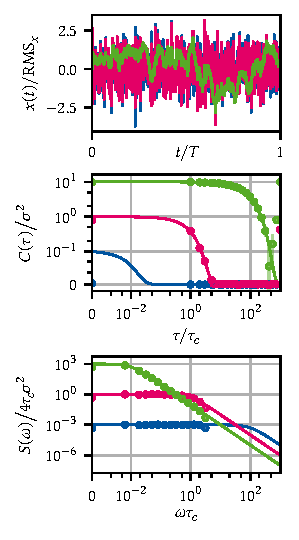
\includegraphics{img/pdf/spectrometer/lorentzian_psdcorr}
    \caption[\imgsource{img/py/spectrometer/lorentz.py}]{
        Ornstein-Uhlenbeck process.
        Simulated time traces (top), autocorrelation function (middle), \gls{psd} (bottom) of the Ornstein-Uhlenbeck process.
        Top: Simluated time traces using the algorithm presented in \cref{ch:ff:time_domain_methods}.
        The data are normalized to the computed \gls{rms} (equal to $\sigma$ in the continuous case).
        Middle: Theoretical autocorrelation function (\cref{eq:speck:ou:autocorrelation}, solid lines) and computed from the simulated data averaged over \num{e3} traces (circles, subset of points).
        Error bars indicate the standard error of the mean, axes are scaled with respect to the parameters of the magenta data, and data are plotted on an $\asinh$-scale.
        Bottom: Theoretical \gls{psd} (\cref{eq:speck:ou:psd}, solid lines) and periodograms computed from the simulated data using \code{scipy.signal.periodogram()}, \cf \cref{eq:speck:periodogram}, averaged over \num{e3} traces (circles, subset of points).
        Axes are again scaled with respect to the parameters of the magenta data and plotted on an $\asinh$-scale.
        Parameters are $\tau_c = \dt\times\{\num{e-2},\num{e0},\num{e2}\}$ and $\sigma^2=\sqrt{\tau_c}/4$ for blue, magenta, and green data, respectively.
    }
    \label{fig:speck:psdcorr}
\end{marginfigure}

To become familiar with the quantities $C(\tau)$ and $S(\omega)$, consider the Ornstein-Uhlenbeck process~\cite{Uhlenbeck1930}, the only stationary Gaussian Markovian stochastic process~\cite{VanKampen1976}.
The autocorrelation function of the Ornstein-Uhlenbeck process is given by
\begin{align}\label{eq:speck:ou:autocorrelation}
    C(\tau) = \sigma^2\e^{-\flatfrac{\tau}{\tau_c}},
\end{align}
with $\sigma$ the \gls{rms} and $\tau_c$ the correlation time of the process.
The \gls{psd} in turn is the Lorentzian function
\begin{align}\label{eq:speck:ou:psd}
    S(\omega) = \frac{2\sigma^2\tau_c}{1 + (\omega\tau_c)^2}.
\end{align}
For a given discretization time step \dt and hence bandwidth $\omega\in [0, \pi\fs]$, the Ornstein-Uhlenbeck process interpolates between perfectly uncorrelated, white noise ($\flatfrac{\dt}{\tau_c}\to\infty, S(\omega) = 2\tau_c\sigma^2$), correlated, pink noise ($\flatfrac{\dt}{\tau_c}\gg 1, S(\omega) = \flatfrac{2\sigma^2}{\tau_c\omega^2}$), and perfectly correlated, quasistatic noise ($\flatfrac{\dt}{\tau_c}\to 0, S(\omega) = \sigma^2\delta(\omega)$).
\Cref{fig:speck:psdcorr} depicts simulated data and its autocorrelation function and \gls{psd} for exemplary parameters: in the white noise limit ($\tau_c = \num{e-2}\dt$, blue), in the intermediate regime ($\tau_c = \dt$, magenta), and in the correlated regime ($\tau_c = \num{e+2}\dt$, green).
From the time series plot at the top it becomes clear that the \gls{rms} alone is insufficient to describe the properties of noisy signals as the curves differ significantly despite being normalized to their \gls{rms}.
The autocorrelation functions averaged over \num{e3} realizations of the noisy signals as well as their theoretical (continuous) value, \cref{eq:speck:ou:autocorrelation}, are plotted in the middle panel, normalized to $\tau_c=\dt$ and $\sigma^2=\flatfrac{\dt}{4}$.
For the white noise limit (blue), correlations are too short to be resolved with the given time discretization.
The correlations decay to $\e\inverse$ at $\flatfrac{\tau}{\tau_c}=\num{e-2},\num{e0},\num{e+2}$, respectively.
Finally, the bottom panel shows the \gls{psd}, \cref{eq:speck:ou:psd}, and its periodogram estimate, again averaged over \num{e3} realizations of the signal and normalized to $\tau_c=\dt$ and $\sigma^2=\flatfrac{\dt}{4}$.
The cross-over from white to pink \gls{psd} occurs at $\omega = \tau_c$.
While the simulated data for $\tau_c = \num{e-2}\dt$ appears perfectly white, that for $\tau_c = \num{e2}\dt$ appears perfectly \oneoverf-like because the spectrum is only white below the smallest resolvable frequency $\df = T\inverse$.

Having gotten an intuition for the quantities $C(\tau)$ and $S(\omega)$, let us move on to see how the latter may be obtained from time series data.
\Cref{eq:speck:psd:definition} represents the starting point for the experimental spectrum estimation procedure.
Instead of a continuous signal $x(t), t\in [0, T]$, consider its discretized version\sidenote{
    We only discuss the problem of equally spaced samples here.
    Variants for spectral estimation of time series with unequal spacing exist~\cite{Lomb1976,Scargle1982}.
}
\begin{align}\label{eq:speck:signal:discrete}
    x_n \qc n\in\lbrace 0, 1, \dotsc, N - 1\rbrace
\end{align}
defined at times $t_n = n\dt$ with $T = N\dt$ and where $\dt = \fs\inverse$ is the sampling interval (the inverse of the sampling frequency \fs).
Invoking the ergodic theorem,\sidenote{
    Note that the limit of perfectly correlated noise, $S(\omega)\propto\delta(\omega)$, technically does \emph{not} correspond to an ergodic process because $C(\tau)=\text{const.}\,\forall\tau\in(-\infty,\infty)$.
    In practice, this is always a mathematical idealization and the spectrum is actually better described by a nascent $\delta$-function with a small but finite width.
}
we can replace the long-term average in \cref{eq:speck:psd:definition} by the ensemble average over $M$ realizations of the noisy signal, $\lbrace x_n\gth{m}\rbrace_m$ and write
\begin{align}\label{eq:speck:psd:bartlett}
    S_n &= \frac{1}{M} \sum_{m=0}^{M-1} \abs{\hat{x}_n\gth{m}}^2 \\
        &= \frac{1}{M} \sum_{m=0}^{M-1} S_n\gth{m}
\end{align}
where $\hat{x}_n\gth{m}$ is the discrete Fourier transform of $x_n\gth{m}$, we defined the \emph{periodogram} of $x_n\gth{m}$ by
\begin{align}\label{eq:speck:periodogram}
    S_n\gth{m} = \abs{\hat{x}_n\gth{m}}^2,
\end{align}
and $S_n$ is an \emph{estimate} of the true \gls{psd} sampled at the discrete frequencies $\omega_n = \flatfrac{2\pi n}{T} \in 2\pi\times\lbrace\flatfrac{-\fs}{2}, \dotsc, \flatfrac{\fs}{2}\rbrace$.\sidenote{
    We blithely disregard integer algebra issues occuring here for conciseness and leave it as an exercise for the reader to figure out what the exact bounds of the set of $\omega_n$ are.
}
\Cref{eq:speck:psd:bartlett} is known as Bartlett's method~\cite{Bartlett1948} for spectrum estimation.\sidenote{
    \label{sidenote:continuum_limit}
    By taking the limit $M\to\infty$ one recovers the true \gls{psd}, \[\lim_{M\to\infty}S_n = S(\omega_n).\]
    The continuum limit is as always obtained by sending $\dt\to 0, N\to\infty, N\dt=\text{const}$.
}

To better understand the properties of this estimate, let us take a look at the parameters $\dt$, $N$, and $M$.
The sampling interval $\dt$ defines the largest resolvable frequency by the Nyquist sampling theorem,
\begin{align}\label{eq:speck:f_max}
    \fmax = \frac{\fs}{2} = \frac{1}{2\dt}.
\end{align}
In turn, the number of samples $N$ determines the frequency resolution $\df$, or smallest resolvable frequency,
\begin{align}\label{eq:speck:f_min}
    \fmin = \df = \frac{1}{T} = \frac{1}{N\dt} = \frac{\fs}{N}.
\end{align}
Lastly, $M$ determines the variance of the set of periodograms $\bigl\lbrace S_n\gth{m}\bigr\rbrace_{i=0}^{M-1}$ and hence the accuracy of the estimate $S_n$.

In practice, the ensemble realizations $i$ are of course obtained sequentially, implying that one acquires a time series of data $x_n, n\in\lbrace0, 1, \dotsc, NM - 1\rbrace$ and partitions these data into $M$ sequences of length $N$.
It becomes clear, then, that the Bartlett average (\cref{eq:speck:psd:bartlett}) trades spectral resolution (larger $N$) for estimation accuracy (larger $M$) given the finite acquisition time $T = NM\dt$.

An improvement in data efficiency can be achieved using Welch's method~\cite{Welch1967}.
To see how, we first need to discuss spectral windowing.

\section{Window functions}\label{sec:speck:theory:windows}
Partitioning a signal $x_n$ into $M$ sections $x_n\gth{m}$ of length $N$ is mathematically equivalent to multiplying the signal with the rectangular \emph{window function} given by\sidenote{
    This window is also known as the boxcar or Dirichlet window.
}
\begin{align}\label{eq:speck:window:boxcar}
    w_n\gth{m} =
    \begin{dcases}
        1 &\qif* (m - 1) N \leq n < m N\qand \\
        0 &\qelse*
    \end{dcases}
\end{align}
so that $x_n\gth{m} = x_n w_n\gth{m}$.
Now recall that multiplication and convolution are duals under the Fourier transform, implying that
\begin{align}\label{eq:speck:window:ft_pairs}
    \hat{x}_n\gth{m} = \hat{x}_n \ast \hat{w}_n\gth{m},
\end{align}
where the Fourier representation of the rectangular window\sidenote{
    $\sinc(x) = \flatfrac{\sin(x)}{x}$.
}
\begin{align}
    \hat{w}_n\gth{m} &= \hat{w}_n \e^{-\i(m - \flatfrac{1}{2})\omega_n T}, \label{eq:speck:window:boxcar:fourier}\\
             \hat{w}_n &= T\sinc\left(\frac{\omega_n T}{2}\right). \label{eq:speck:window:boxcar:fourier:unshifted}
\end{align}
\begin{marginfigure}
    \centering
    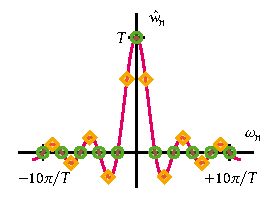
\includegraphics{img/pdf/spectrometer/rect}
    \caption[\imgsource{img/py/spectrometer/pyspeck.py}]{
        The Fourier representation of the rectangular window in continuous time (solid line) and for discrete frequencies $\omega_n = \flatfrac{2\pi n}{T}$ (circles).
        Introducing a phase shift, that is, shifting the window with respect to the signal in time, effectively shifts $\omega_n \to \omega_{n+\eta}$ as indicated for $\eta=\flatfrac{1}{2}$ (diamonds).
        This incurs scalloping loss.
    }
    \label{fig:speck:boxcar_fourier}
\end{marginfigure}
\begin{marginfigure}
    \centering
    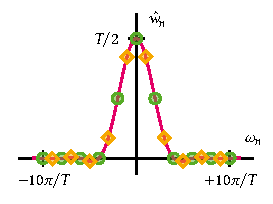
\includegraphics{img/pdf/spectrometer/hann}
    \caption[\imgsource{img/py/spectrometer/pyspeck.py}]{
        The Fourier representation of the Hann window in continuous time (solid line) and for discrete frequencies $\omega_n$ (circles).
        Diamonds indicate discrete sampling when the window completely out of phase with the signal (\cf \cref{fig:speck:boxcar_fourier}).
    }
    \label{fig:speck:hann_fourier}
\end{marginfigure}
\Cref{fig:speck:boxcar_fourier} shows the unshifted rectangular window $\hat{w}_n$ in Fourier space.
We can hence understand the Fourier spectrum of $x_n\gth{m}$ as sampling $\hat{x}_n$ with the probe $\hat{w}_n\gth{m}$.
However, while in the continuum limit (\cref{sidenote:continuum_limit}) \cref{eq:speck:window:boxcar:fourier:unshifted} tends towards $\delta(\omega_n)$ and thus will produce a faithful reconstruction of the true spectrum, the finite frequency spacing $\df$ of discrete signals and finite observation length $T$ introduce a finite bandwidth of the probe as well as \emph{sidelobes}.
These effects induce what is known as \emph{spectral leakage} and \emph{scalloping loss}~\cite{Harris1978,Koopmans1995} and lead to artifacts and deviations of the spectrum estimator $S_n$ from the true spectrum $S(\omega_n)$.

For this reason, a plethora of \emph{window functions} have been introduced to mitigate the effects of spectral leakage.
Key properties of a window are the spectral bandwidth (center lobe width) and sidelobe amplitude between which there typically is a tradeoff.\sidenote{
    Wikipedia gives a good overview of existing window functions~\cite{WindowFunctionWiki}.
}
A window frequently used in spectral analysis is the Hann window~\cite{Nuttall1981},
\begin{align}\label{eq:speck:window:hann}
    w_n\gth{m} =
    \begin{dcases}
        \sin^2\left(\frac{\pi n}{N}\right) &\qif* (m - 1)N\leq n < mN\qand \\
        0 &\text{else},
    \end{dcases}
\end{align}
with the Fourier representation of the unshifted window,
\begin{align}\label{eq:speck:window:hann:fourier_unshifted}
    \hat{w}_n &= \frac{T}{2}\sinc\left(\frac{\omega_n T}{2}\right)\times
                 %  \frac{1}{2(1 - \flatfrac{\omega_n T}{2\pi})(1 + \flatfrac{\omega_n T}{2\pi})},
                    \frac{1}{1 - \left(\flatfrac{\omega_n T}{2\pi}\right)^2}
\end{align}
shown in \cref{fig:speck:hann_fourier}.
The favorable properties of the Hann window are apparent when compared to the rectangular window in \cref{eq:speck:window:boxcar:fourier:unshifted} and \cref{fig:speck:boxcar_fourier}; the sidelobes are quadratically suppressed while the center lobe is only slightly broadened.

Another favorable property of the Hann window is that $w_0\gth{0} = w_{N-1}\gth{0} = 0$.
This suppresses detrimental effects arising from a possible discontinuity ($x_0\gth{0}\neq x_{N-1}\gth{0}$) at the edge of a data segment related to the discrete Fourier transform, which assumes periodic data.\sidenote{
    Although this can usually also be achieved approximately by detrending the data before performing the Fourier transform, which is a good idea in any case.
}

\section{Welch's method}\label{sec:speck:theory:welch}
Contemplating \cref{eq:speck:window:hann}, one might come to the conclusion that using a window such as this is not very data efficient in the sense that a large fraction of samples located at the edge of the window is strongly suppressed and hence does not contribute significantly to the spectrum estimate.
To alleviate this lack of efficiency, one can introduce an overlap between adjacent data windows.
That is, instead of partitioning the data $x_n$ into $M$ non-overlapping sections of length $N$, one shifts the $m$th window forward by $-mK$ with $K>0$ the overlap.
Finally, the periodogram (\cref{eq:speck:periodogram}) is computed for each window and subsequently averaged to obtain the spectrum estimator (\cref{eq:speck:psd:bartlett}).

This method of spectrum estimation is known as Welch's method~\cite{Welch1967}.
One can show~\cite{Welch1967} that the correlation between the periodograms of adjacent, overlapping windows is sufficiently small to avoid a biased estimate.
The overlap naturally depends on the choice of window; a typical value for the Hann window $K = \flatfrac{N}{2}$ with which one would obtain $M = \flatfrac{2L}{N} - 1$ windows for data of length $L$.\sidenote{
    Again neglecting integer arithmetic issues.
}
\begin{figure}
    \centering
    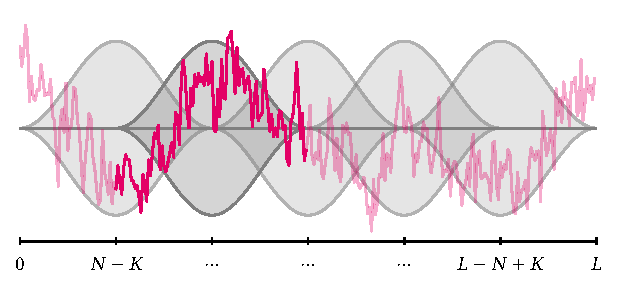
\includegraphics[width=\textwidth]{img/pdf/spectrometer/welch}
    \caption[\imgsource{img/py/spectrometer/pyspeck.py}]{
        Illustration of Welch's method for spectrum estimation.
        The data (pink) of length $L$ is partitioned into $K = \flatfrac{2L}{N} - 1$ segments of length $N$.
        Each segment is multiplied with a window function (gray) which reduces spectral leakage and other artifacts.
        A finite overlap $K$ between adjacent windows (gray) ensures efficient sample use.
    }
    \label{fig:speck:welch}
\end{figure}

\Cref{fig:speck:welch} conceptually illustrates Welch's method for a trace of \oneoverf noise with $L = 300$ samples in total.
Choosing the Hann window and an overlap of \qty{50}{\percent} results in $M=5$ segments for a window length of $N=100$.
The data in the second window is highlighted.

\section{Parameters \& Properties of the \acrshort{psd}}\label{sec:speck:theory:welch:parameters}
\begin{margintable}[*-7]
    \centering
    \footnotesize
    \caption[Overview of spectrum estimation parameters]{
        Overview of spectrum estimation parameters.
        The parameters can be assigned into four groups
        \begin{enumerate*}[
            before=\unskip{: }, itemjoin={{, }}, itemjoin*={{, and }}
        ]
            \item \acrshort{daq} parameters configuring the \acrlong{daq} device
            \item Welch parameters specifying the periodogram averaging
            \item Spectrum properties induced by the above
            \item External parameters unrelated to the others
        \end{enumerate*}.
    }
    \label{tab:speck:theory:parameters}
    \renewcommand{\arraystretch}{1.1}
    \begin{tabularx}{\marginparwidth}{ c l }
        \multicolumn{2}{l}{1. \acrshort{daq} parameters} \\
        \toprule
        $L$ & Total number of samples \\
        \fs & Sample rate \\
        [0.5ex]
        \multicolumn{2}{l}{2. Welch parameters} \\
        \toprule
        $K$ & Number of overlap samples \\
        $N$ & Number of segment samples \\
        $M$ & Number of Welch segments \\
        [0.5ex]
        \multicolumn{2}{l}{3. Spectrum parameters} \\
        \toprule
        \fmin & Smallest resolvable frequency \\
        \fmax & Largest resolvable frequency \\
        \multicolumn{2}{l}{4. Miscellaneous parameters} \\
        \toprule
        $O$ & Number of outer averages \\
    \end{tabularx}
\end{margintable}
We are now in a position to discuss how the various parameters of a time series relate to both the physical parameters of the resulting spectrum estimate and to each other.
To this end, we will go through the typical procedure of acquiring a spectrum estimate using Welch's method chronologically.

To acquire data using some form of (digital) \gls{daq}, one usually needs to specify two parameters first: the total number of samples to be acquired, $L$, and the sample rate \fs.
This results in a measurement of duration $T = L\dt$ where $\dt = \fs\inverse$ as previously mentioned.
The choice of \fs already induces an upper bound on the first parameter characterizing the \gls{psd} estimate: the largest resolvable frequency $\fmax\leq\flatfrac{\fs}{2}$ (\cf \cref{eq:speck:f_max}, but note that we allow \fmax to be smaller than half the sample rate in anticipation of hardware constraints).
Next, we choose a number of Welch averages, $M$, \ie, data partitions, and their overlap, $K$.
In doing so, one fixes the number of samples per partition $N$ and thereby induces the lower bound on the second parameter characterizing the \gls{psd} estimate: the frequency spacing $\df = \flatfrac{1}{N} \leq \fmin$ (\cf \cref{eq:speck:f_min}).\sidenote[][*-3]{
    Technically, the smallest resolvable frequency in a \gls{fft} is zero, of course. But as data is typically detrended (a constant or linear trend subtracted) before computation of the periodogram, the smallest \emph{meaningful} frequency is given by \fmin.
}
% TODO: be consistent in use of segment vs partition?
Finally, we can introduce a number of \emph{outer} averages $O$, that is, the number of data batches that are acquired.
While not directly related to Welch's method, choosing $O > 1$ can, for instance, help achieve a certain variance if the number of samples per batch, $L$, is limited by the \acrlong{daq} hardware, or simply allow for updating the spectrum estimate as data is being acquired.
\Cref{fig:speck:theory:parameters} shows the relationships of the various parameters among each other.
In \cref{subsec:speck:software:design:daq}, I lay out how these inter-dependencies are implemented in software.

\begin{figure}
    \centering
    \begin{tikzpicture}[
    >=stealth,
    auto,
    box/.style={
        draw,
        rectangle,
        rounded corners,
        thick,
        align=center,
        inner sep=2mm,
%        drop shadow,
    },
    float1/.style={box, fill=RWTHmagenta25, text=RWTHmagenta100},
    float2/.style={box, fill=RWTHmagenta10, text=RWTHmagenta75},
    int1/.style={box, fill=RWTHgreen25, text=RWTHgreen100},
    int2/.style={box, fill=RWTHgreen10, text=RWTHgreen75},
    int3/.style={box, fill=RWTHblack10, text=RWTHblack100},
]

    % Central node: nperseg
    \node[int1] (nperseg) {$N$};

    % Frequency branch: relative to nperseg, all nodes placed at the same x-coordinate.
    \node[float1, above left=1cm of nperseg, anchor=center] (fs) {\fs};
    \node[float1, below left=1cm of nperseg, anchor=center] (df) {\df};
    \node[float2, left=of fs] (fmax) {\fmax};
    \node[float2, left=of df] (fmin) {\fmin};

    % Segmentation branch: relative to nperseg
    \node[int2, right=of nperseg] (npts) {$L$};
    \node[int2, above right=of npts, anchor=center] (noverlap) {$K$};
    \node[int2, below right=of npts, anchor=center] (nseg) {$M$};

    % Stand-alone node for n_avg
    \node[int3, above=1cm of $(npts)!0.5!(nperseg)$] (navg) {$O$};

    % Draw frequency branch arrows
    \draw[->] (nperseg) -- (fs);
    \draw[->] (nperseg) -- (df);
    \draw[<->] (df) to[bend left=45] (fs);
    \draw[->] (fs) to[bend right=45] (fmax);
    \draw[->] (df) to[bend left=45] (fmin);
    \draw[<->] (fs) -- (nperseg);
    \draw[<->] (df) -- (nperseg);

    % Draw segmentation branch arrows (nperseg, noverlap, and n_seg together inform n_pts)
    \draw[<->] (nperseg) -- (npts);
    \draw[->] (noverlap) -- (npts);
    \draw[->] (nseg) -- (npts);

    % n_avg remains independent (no arrows drawn)

\end{tikzpicture}

    \caption[\imgsource{img/tikz/spectrometer/daq_settings.tex}]{
        Relationships of data acquisition parameters (\cf \cref{tab:speck:theory:parameters,tab:speck:software:parameters}, with arrows indicating dependencies.
        $N$, \fs, and \df are the central quantities defining the estimated spectrum's properties.
        From \fs and \df follow (bounds for) \fmax and \fmin.
        From $N$, together with $K$ and $M$, follows $L$, the total number of samples per data batch.
    }
    \label{fig:speck:theory:parameters}
\end{figure}

To conclude this chapter, let us discuss some of the properties of stochastic processes and their autocorrelation function and \gls{psd}.
Consider again the process $x(t)$.
We say $x(t)$ is \emph{Gaussian} if $x(t)\sim\mathcal{N}(\mu, \sigma^2)\,\forall t$, meaning that the value of $x(t)$ at a given point in time follows a normal distribution with some mean $\mu$ and variance $\sigma^2$ over multiple realizations of the process.
In this case, its statistical properties are fully described by the autocorrelation function $C(\tau)$ and \gls{psd} $S(\omega)$.
This is because only the first two cumulants of a Gaussian distribution are nonzero~\cite{Fox1978}.
For the purpose of noise estimation, the assumption of Gaussianity is a rather weak one as the noise typically arises from a large ensemble of individual fluctuators and is therefore well approximated by a Gaussian distribution by the central limit theorem~\cite{Krzywda2020}.\sidenote{
    As an example, consider electronic devices, where voltage noise is thought to arise from a large number of defects and other charge traps in oxides being populated and depopulated at certain rates $\gamma$. The ensemble average over these so-called \glspl{tlf} then yields the well-known \oneoverf-like noise spectra~\cite{Schriefl2006,Beaudoin2015} (at least for a large density~\cite{Mehmandoost2024}).
}
Even if $x(t)$ is not perfectly Gaussian, non-Gaussian contributions can be seen as higher-order contributions if viewed from the perspective of perturbation theory, and therefore the \gls{psd} still captures a significant part of the statistical properties.
For this reason, the \gls{psd} is the central quantity of interest in noise spectroscopy.
Let us just note at this point that techniques to estimate higher-order spectra (or \emph{polyspectra}) exist~\cite{Chandran1994,Norris2016,Szankowski2017}.

For real signals $x(t)\in\mathbb{R}$, the autocorrelation function $C(\tau)$ is an even function, while for $x(t)\in\mathbb{C}$ its real part is even and its complex part odd.
From this it immediately follows that for real $x(t)$ $S(\omega)$ is also an even function and one therefore distinguishes the \emph{two-sided} \gls{psd} $S^{(2)}(\omega)$ defined over $\mathbb{R}$ from the \emph{one-sided} \gls{psd} $S^{(1)}(\omega) = 2 S^{(2)}(\omega)$ defined only over $\mathbb{R}^+$.
Complex $x(t)$ such as those generated by \glspl{lia} after demodulation in turn have asymmetric, two-sided \glspl{psd}.
In this chapter so far, we have implicitly employed the two-sided definition, but in the software package presented in \cref{ch:speck:software}, two-sided spectra are used only for complex data since they contain redundant information for real data.
